% !TEX root = ../main.tex

In diesem Kapitel wird auf die Vorgehensweise, wie die Visualisierung implementiert wird, eingegangen und die genutzten Technologien werden vorgestellt. Der Abschnitt~\ref{subchap:app-struct} behandelt die Struktur der Applikation sowie die verwendeten Klassen. %, verdeutlicht in der Abbildung~\ref{fig:uml-app} in einem \emph{UML}-Diagramm.
Die Klasse~\emph{Model} stellt dabei das Kernelement der Applikation dar und wird ausführlicher betrachtet.
In dieser Klasse wird aus dem gerichteten Graphen von Kategorien der Kategorienbaum konstruiert und die gefilterte Ähnlichkeitsmatrix der Artikelvergleiche gespeichert.
Im Abschnitt~\ref{subchap:external-libs} wird ausgeführt, welche Bibliotheken in der Arbeit genutzt werden.


\section{Programmstruktur} \label{subchap:app-struct}
Die Applikation ist eine in \emph{c++} und \emph{OpenGL} realisierte Visualisierung mit verschiedenen Bibliotheken, welche in Abschnitt \ref{subchap:external-libs} erläutert werden.
Für die Architektur von Applikationen der Informationsvisualisierung existieren unterschiedliche Referenzmodelle, wie von Chi~\cite{EdHuaiHsinChi}, Card~\cite{card1999readings} oder Tang~\cite{Tang2004}.
Diese Arbeit orientiert sich am Referenzmodell nach Card et al.~\cite{card1999readings}, welches in der Abbildung~ \ref{fig:ref-model} dargestellt ist.
Dieses Modell veranschaulicht die verschiedenen Schritte, die benötigt werden, um aus den Rohdaten eine Visualisierung zu konstruieren.
Der erste Schritt besteht aus dem Sammeln der Rohdaten.
Im zweiten Schritt, der Transformation der Daten, werden die Rohdaten in eine strukturierte Datenform gebracht.
Die strukturierten Daten werden als eine visuelle Repräsentation abgebildet.
Dieser Schritt wird als \emph{visuelle Zuordnung} (\emph{Visual Mapping}) bezeichnet.
Der letzte Schritt ist die Darstellung der visuellen Repräsentation auf der Bildoberfläche.
Wie in der Abbildung~\ref{fig:ref-model} dargestellt, ist der Nutzer im Stande, während des gesamten Ablaufs einzugreifen und Änderungen vorzunehmen.
Das Modell ermöglicht dabei eine differenziertere Ansicht der visuell abstrakt dargestellten Daten sowie die Interaktion mit ihnen.

% Die Abbildung~\ref{fig:uml-app} zeigt ein UML-Diagramm der Applikation mit ihren Klassen.
% Zur Übersicht werden die Klassen auf ihre Kernfunktionen reduziert.
Die Klasse~\emph{Model} stellt die visuelle Struktur dar und ist das Kernelement der Anwendung.
In ihr wird sowohl der Kategorienbaum konstruiert, als auch die aus der Datenbank gefilterte Ähnlichkeitsmatrix gespeichert.
Des Weiteren kann die Klasse die Anordnung der Knoten bestimmen und den Kategorienbaum erweitern.
Die Klasse~\emph{Renderer} ist die Schnittstelle zur Grafikkarte.
Diese ist für die Darstellung der Knoten und Kanten auf der Bildoberfläche zuständig und realisiert einige der Interaktionen der Anwendung, wie die der Verschiebung, Vergrößerung oder der Rotation der dargestellten Knoten und Kanten.
In den Klassen~\emph{Gui} und~\emph{View} sind die grafischen Benutzeroberflächen implementiert.
Die Elemente~(c), die Suchleiste~(d) und der Regler zur Bestimmung des Schwellwerts der Ähnlichkeiten sind in der Klasse~\emph{Gui} implementiert.
Die statistische Zusammenfassung~(b) aus der Abbildung~\ref{fig:small-start} und die Beschriftungen der Knoten sind in der Klasse~\emph{View} implementiert.


% beide grafiken zu MVC und refMODEL
\begin{figure}
    \centering
    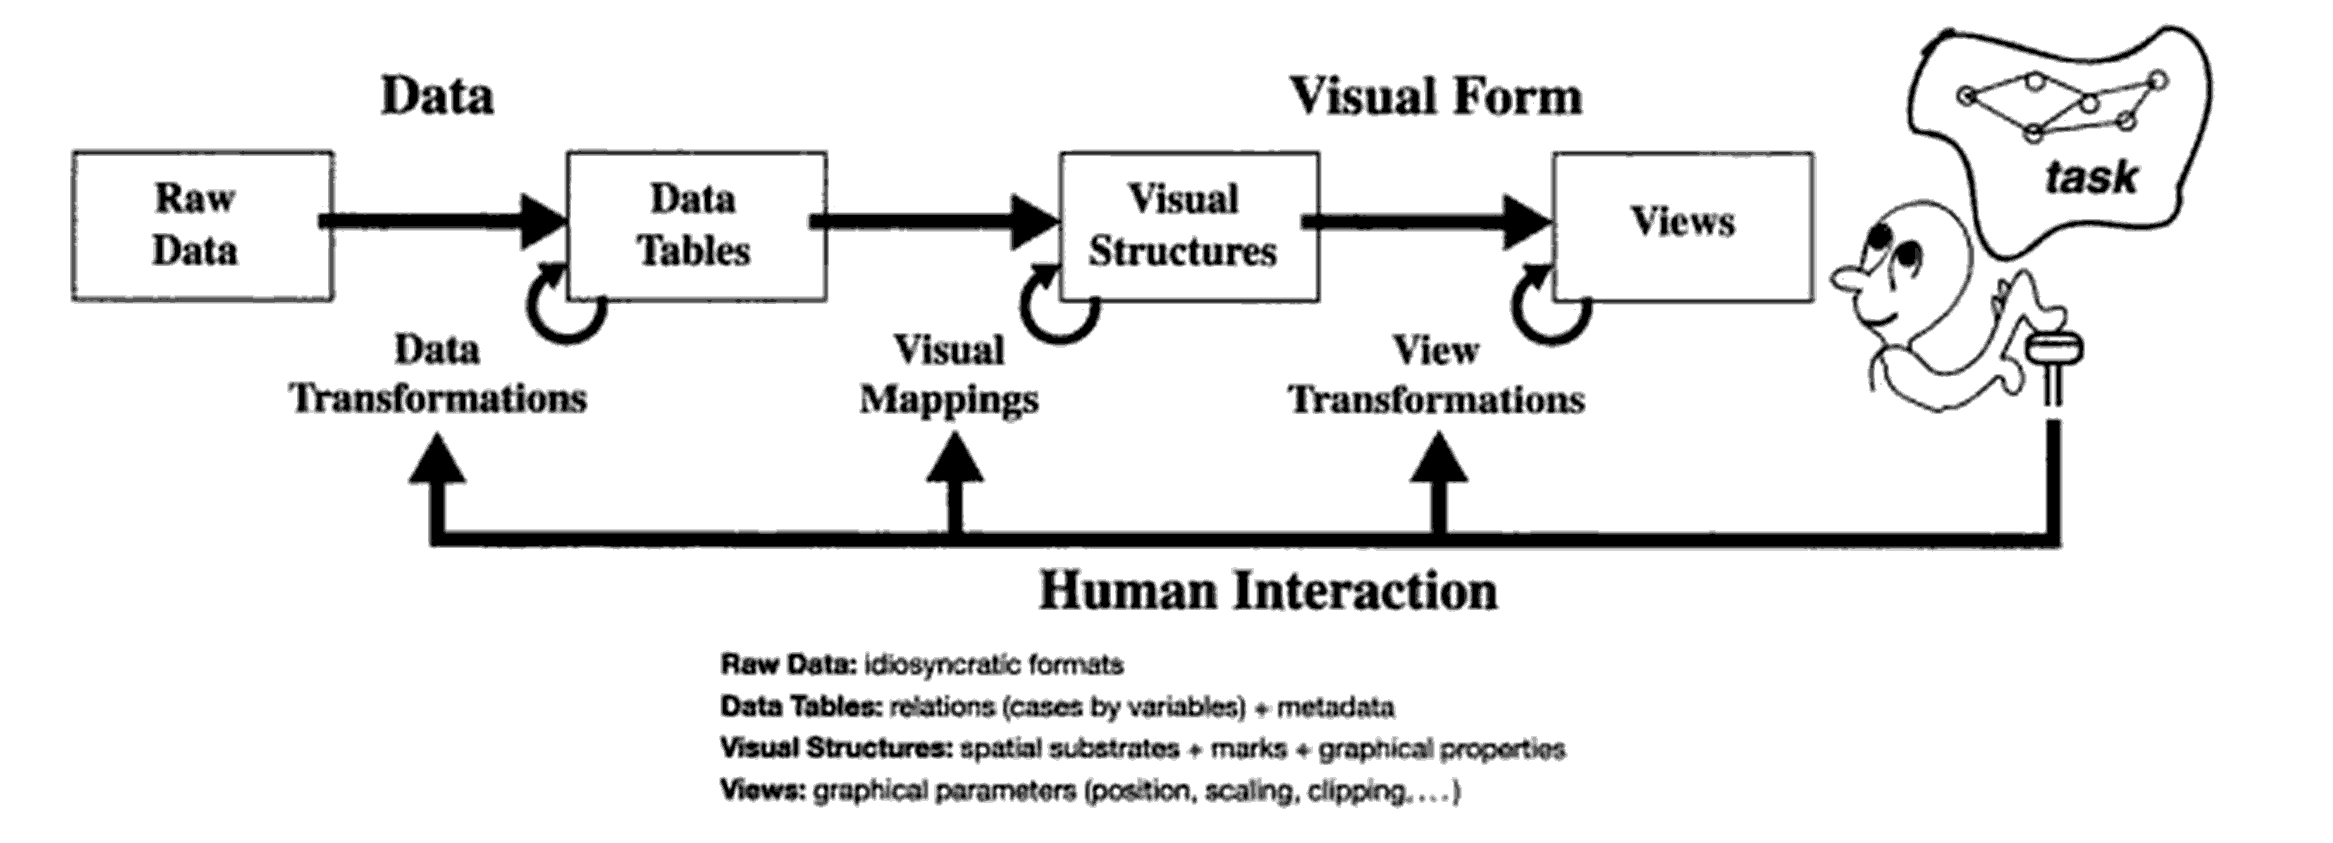
\includegraphics[width=\textwidth]{images/card-model}
    \caption{Referenzmodell nach Card et al. \cite{card1999readings} }
    \label{fig:ref-model}
\end{figure}


% grafik mit schema eines Baumes und doppelten kanten zu veranschaulichung

\paragraph{Kernfunktionen}
Im nachfolgenden Abschnitt wird auf die Kernfunktion, die Konstruktion des Kategorienbaums und die Klasse~\emph{Model} eingegangen.
Wie bereits im Abschnitt~\ref{subchap:layout} angedeutet, wird eine Methode entwickelt, die aus den gerichteten Verknüpfungen des Kategoriengraphen, die der Datenbank entnommen werden, einen Baum konstruiert.

Die unterschiedlichen Schritte erfüllen dabei bestimmte Voraussetzungen:\\
Für die Konstruktion eines Kategorienbaums ist es möglich, jede Kategorie als Ausgangspunkt festzulegen und somit als Wurzelkategorie zu bestimmen.
Dadurch wird die Möglichkeit geschaffen, direkt in ein Themengebiet einzusteigen und dessen Unterkategorien zu erkunden.
Damit die Kategorien des Baums eine hierarchische Struktur bilden, werden mit der Breitensuche Unterkategorien des Kategoriengraphen traversiert.
Hinzu kommt, dass weder Schleifen im Kategorienbaum existieren noch Kategorien mehrfach enthalten sein dürfen.
Um für die ausgewählte Startkategorie nicht jede Unterkategorie traversieren zu müssen, bedarf es einer Möglichkeit, die Traversierung abzubrechen.
Deshalb wird die Konstruktion des Kategorienbaums mit der iterativen Tiefensuche nach Korf~\cite{korf1985depth} realisiert.

Ausgehend von der gewählten Wurzelkategorie und der angegebenen Tiefe durch den Nutzer werden die Unterkategorien der Wurzelkategorie mit der iterativen Tiefensuche erkundet und dem Kategorienbaum hinzugefügt.
Bei einer Tiefe von 0 als Startpunkt wird der Kategoriengraph aufsteigend bis zu einer durch den Nutzer festgesetzten Tiefe mehrfach traversiert.
Die iterative Tiefensuche erkundet zuerst die direkten Unterkategorien der Ausgangskategorie bevor weitere Knoten besucht werden.
Somit werden dem Kategorienbaum erst die Unterkategorien einer Ebene hinzugefügt, bevor der Algorithmus die Kategorien der nächsten Tiefe erkundet.
Auf diese Weise werden die Kategorien in der selben Reihenfolge wie bei einer Breitensuche erkundet.
Folglich werden dem Baum kontinuierlich Kategorien tieferer Abstraktionsebenen hinzugefügt.
Dies ist notwendig, um die Hierarchie beizubehalten.
Ist die festgelegte Tiefe durch mehrfache Iteration erreicht, ist der Kategorienbaum konstruiert.
Wie bereits zu Beginn des Kapitels~\ref{chap:visualization} erläutert, entspricht der konstruierte Kategorienbaum einer Interpretation des Kategoriengraphen ausgehenden von einer bestimmten Wurzelkategorie .

% pseudocode!! 
% Im folgenden Pseudocode wird der Algorithmus dargelegt.

% % evtl. dopplung mit vis kapitel
% In der Abbildung~\ref{fig:abstract-tree} werden ein schematischer Kategoriengraph und zwei verschiedene Kategorienbäume mit unterschiedlichen Wurzelkategorien dargestellt.
% Die Abbildung zeigt, dass mit diesem Ansatz keine eindeutige Hierarchie dargestellt werden kann.


% \begin{figure}
%     \centering
%     
\includegraphics{images/todobild.pdf}
%     \caption{Schematische Darstellung eines Auszugs des Kategoriengraphen und eines Kategorienbaums.}
%     \label{fig:abstract-tree}
% \end{figure}

%\begin{figure}
%    \centering
%    
\includegraphics{images/todobild.pdf}
%    \caption{UML-Diagramm der Visualisierung}
%    \label{fig:uml-app}
%\end{figure}


\section{Externe Bibliotheken}\label{subchap:external-libs}

In der Arbeit werden eine Vielzahl an Bibliotheken genutzt, die unterschiedliche Aufgaben übernehmen.
Im folgenden Abschnitt werden die Bibliotheken kurz erläutert.
Zudem wird darauf eingegangen, welche Funktionalitäten sie der Applikation hinzufügen.
Auf die Datenbank~\emph{FastDB} und die Datenbankschnittstelle \emph{WikiDB} wird an dieser Stelle nicht weiter eingegangen, da sie in dem Kapitel~\ref{chap:daten} ausführlich beschrieben sind.

\paragraph{Boost Graph Library}
Die \emph{Boost Graph Library} (\emph{BGL}) \footnote{\url{http://www.boost.org/doc/libs/1_65_1/libs/graph/doc/}} spielt eine wesentliche Rolle bei der Transformation der strukturierten Daten in eine visuelle Repräsentation, die folglich auf der Bildoberfläche dargestellt wird.
Die \emph{BGL} ermöglicht das Speichern der Informationen aus der Datenbank in einer Graphenstruktur.
Die Bibliothek bietet eine Vielzahl an Graphenalgorithmen an; u.~a. für die Traversierung und Anordnung der Knoten oder Kanten.
Die Vielzahl an Funktionalitäten aufzuzählen, die durch die \emph{BGL} angeboten werden, würde den Rahmen dieser Arbeit allerdings übersteigen.
Daher wird nachfolgend nur auf die in dieser Arbeit verwendeten Funktionen eingegangen.
Die \emph{BGL} wird genutzt, um eine Graphendatenstruktur zu Modellierung der Hierarchien der Kategorien zu realisieren.
Dabei lassen sich eine Vielzahl von Einstellungen für die Funktionsweise der Graphendatenstruktur vornehmen.
Beispielsweise ist es möglich festzulegen, ob die Kanten des Graphen ungerichtet oder, wie in dieser Arbeit, gerichtet sind.
Darüber hinaus besteht die Möglichkeit, den Knoten und Kanten des Graphen Eigenschaften wie die Farbe, Titel, Position oder die Gewichtung zuzuweisen.

\paragraph{NanoVG und NanoGUI}
Die Bibliothek \emph{NanoVG} \cite{nanovg} ermöglicht es, angelehnt an das~\emph{HTML-canvas}, grafische Elemente in einem \emph{OpenGl-Context} zu zeichnen.
In dieser Arbeit wird die Bibliothek dazu genutzt, die Kategorienknoten innerhalb des Hauptfensters zu beschriften und den Text der statistischen Zusammenfassung~(b) aus der Abbildung~\ref{fig:small-start} zu zeichnen.
Mit der \emph{NanoVG} lassen sich auch weitere Elemente, wie z.~B. ein Histogramm oder ein Graph, welcher dem Nutzer weitere Informationen über den dargestellten Datensatz liefert, zeichnen.
Die Bibliothek \emph{NanoGUI} \cite{nanogui} wird verwendet, um grafische Benutzeroberflächen zu konstruieren.
Die Elemente~(c) und~(d) aus der Abbildung~\ref{fig:small-start} sind in der Bibliothek implementiert.
Darüber hinaus bietet die \emph{NanoGUI} ein vielseitiges Repertoire an nützlichen Bausteinen, um weitere grafische Benutzeroberflächen für die Applikation zu konstruieren.
